
\begin{figure}
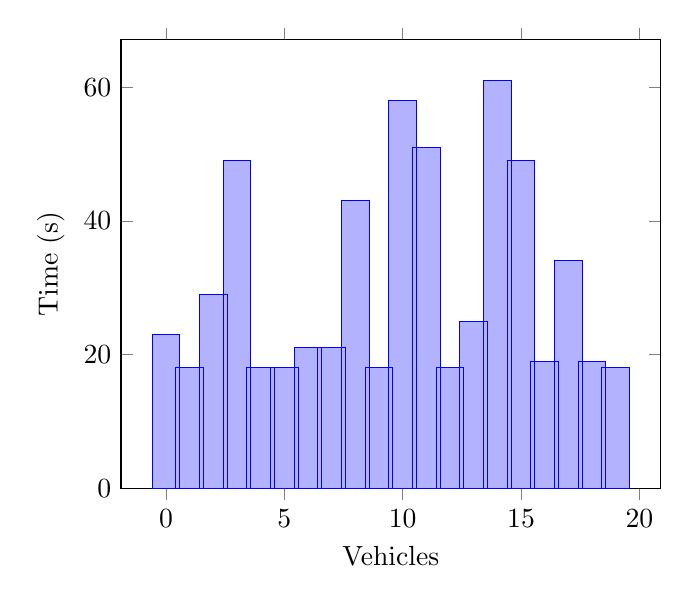
\begin{tikzpicture}
\begin{axis}[
legend style={anchor=west},
xlabel=Vehicles,
ylabel=Time (s),
ymin=0,
ybar,
]
\addplot coordinates {
(0, 23)
(1, 18)
(2, 29)
(3, 49)
(4, 18)
(5, 18)
(6, 21)
(7, 21)
(8, 43)
(9, 18)
(10, 58)
(11, 51)
(12, 18)
(13, 25)
(14, 61)
(15, 49)
(16, 19)
(17, 34)
(18, 19)
(19, 18)
};

\end{axis}
\end{tikzpicture}
\label{tik:100:3_V, 3_V.-60, 1_N}
\caption{100 percent diving with GSC on route $3_V, 3_V.-60, 1_N$}
\end{figure}
